%%% Local Variables:
%%% mode: latex
%%% TeX-master: t
%%% End:

\documentclass{beamer}

\usepackage{beamerthemeMadrid}
\usepackage[makeroom]{cancel}
\usepackage{dsfont}
\usepackage{graphicx,color}
\usepackage{tikz}
\usepackage{tikz-qtree}
\usepackage{MnSymbol,wasysym}

\usetikzlibrary{trees}

\newcommand{\C}{{\mathds{C}}}
\newcommand{\D}{{\mathds{D}}}
\newcommand{\DD}{{\mathcal{D}}}
\newcommand{\T}{{\mathcal{T}}}
\newcommand{\R}{{\mathds{R}}}
\newcommand{\N}{\mathbb{N}}
\newcommand{\F}{\mathbb{F}}
\newcommand{\RR}{\mathbb{R}}
\newcommand{\Z}{\mathbb{Z}}

%\usepackage{mathpazo}
%\usepackage[margin=1in]{geometry}
%\usepackage{mathtools}
%\usepackage{color}
\usepackage{proof}


\usepackage{amsmath}
\usepackage{mathtools}
\usepackage[alphabetic]{amsrefs}
\usepackage{url}
\BibSpec{article}{%
    +{}  { \PrintAuthors}               {author}
    +{,} { \textit}                     {title}
    +{.} { }                            {part}
    +{:} { \textit}                     {subtitle}
    +{,} { \PrintContributions}         {contribution}
    +{.} { \PrintPartials}              {partial}
    +{,} { }                            {journal}
    +{,} { \voltext}                    {volume}
    +{,} { \issuetext}                  {number}
    +{,} { pp.~}                        {pages}
    +{}  { \PrintDatePV}                {date}
    +{,} { }                            {status}
    +{,} { \PrintDOI}                   {doi}
    +{,} { available at \eprint}        {eprint}
    +{}  { \parenthesize}               {language}
    +{}  { \PrintTranslation}           {translation}
    +{;} { \PrintReprint}               {reprint}
    +{.} { }                            {note}
    +{.} {}                             {transition}
    +{}  {\SentenceSpace \PrintReviews} {review}
}
% \bibliographystyle{plain}
\newcommand{\arxiv}[1]{\href{https://arxiv.org/abs/#1}{arXiv:#1}}
\newcommand{\iacr}[1]{\href{https://eprint.iacr.org/#1}{Cryptology ePrint Archive, Report #1}}
\newcommand{\pdflink}[1]{\url{#1}}
\renewcommand{\eprint}[1]{#1}

%\usepackage[colorlinks,citecolor=blue]{hyperref}
%\usepackage{amsthm}
%\newtheorem{theorem}{Theorem} %[section]
%\newtheorem{lemma}[theorem]{Lemma}
%%\newtheorem{proposition}[theorem]{Proposition}
%\newtheorem{corollary}[theorem]{Corollary}
%\newtheorem{example}[theorem]{Example}
%\newtheorem{remark}[theorem]{Remark}
%\newtheorem{definition}[theorem]{Definition}

\newcommand{\eq}[1]{\hyperref[eq:#1]{(\ref*{eq:#1})}}
\renewcommand{\sec}[1]{\hyperref[sec:#1]{Section~\ref*{sec:#1}}}
\newcommand{\thm}[1]{\hyperref[thm:#1]{Theorem~\ref*{thm:#1}}}
\newcommand{\lem}[1]{\hyperref[lem:#1]{Lemma~\ref*{lem:#1}}}
\newcommand{\cor}[1]{\hyperref[cor:#1]{Corollary~\ref*{cor:#1}}}
\newcommand{\itm}[1]{\hyperref[itm:#1]{\ref*{itm:#1}}}
\newcommand{\app}[1]{\hyperref[app:#1]{Appendix~\ref*{app:#1}}}

\newcommand{\nm}[1]{\lVert #1\rVert}
\newcommand{\sem}[1]{[\![ #1 ]\!]}
\newcommand{\bra}[1]{\langle #1 \vert}
\newcommand{\ket}[1]{\vert #1 \rangle}
\newcommand{\tr}[0]{\mathrm{tr}}
\newcommand{\blue}[1]{\textcolor{blue}{#1}}
\newcommand{\cskip}[0]{{\mathbf{skip}}}
\newcommand{\cif}[3]{{\mathbf{if}~#1~\mathbf{then}~#2~\mathbf{else}~#3}}
\newcommand{\cwhile}[2]{{\mathbf{while}~#1~\mathbf{do}~#2}}
\newcommand{\qif}[2]{\mathbf{if}~#1\to #2~\mathbf{fi}}
\newcommand{\qwhile}[2]{\mathbf{while}~#1~\mathbf{do}~#2~\mathbf{od}}
\newcommand{\Var}[0]{\mathrm{Var}}
\newcommand{\Val}[0]{\mathrm{Val}}
\newcommand{\op}[0]{\mathrm{op}}
\newcommand{\In}[0]{\mathrm{In}}
\newcommand{\Obs}[0]{\mathrm{Obs}}
\newcommand{\dist}[0]{\mathrm{dist}}
\newcommand{\Cont}[0]{\mathrm{Cont}}
\newcommand{\dhall}[0]{\mathcal{D}(\mathcal{H}_{all})}
\newcommand{\dhnall}[0]{\mathcal{D}(\mathcal{H})}
\newcommand{\qoh}[0]{\mathcal{QO(H)}}
\newcommand{\qohall}[0]{\mathcal{QO(H_{all})}}
\newcommand{\E}[0]{\mathcal{E}}
\newcommand{\FF}[0]{\mathcal{F}}
\renewcommand{\H}[0]{\mathcal{H}}
\newcommand{\loww}[0]{L\"{o}wner}






\makeatletter
\renewcommand*\env@matrix[1][c]{\hskip -\arraycolsep
  \let\@ifnextchar\new@ifnextchar
  \array{*\c@MaxMatrixCols #1}}
\makeatother


\title[Quantum Hoare Logic and a Ranking Function]{Quantum Hoare Logic and a Ranking Function}
\author[Project CMSC 631]{Shouvanik Chakrabarti, Andrew Fichman, Shaopeng Zhu}
\date{\today}

\begin{document}

\frame{\titlepage}

%\section{Background}
\frame[t]{
\frametitle{Introduction: Structure of the Talk}
\begin{enumerate}
\item Background Knowledge in Quantum Computation
\item Syntax and Semantics of Quantum Programs
\begin{enumerate}
    \item Syntax
    \item Operational Semantics
    \item Denotational Semantics
\end{enumerate}

%\hskip

\item Quantum Hoare Logic
\begin{enumerate}
    \item 
    \item 
\end{enumerate}

%\hskip

\item Linear-Ranking Super Martingale (LRSM): a Ranking Function
\begin{enumerate}
    \item 
    \item 
\end{enumerate}
\end{enumerate}
}

\frame[t]{
\frametitle{Syntax: From Classical to Quantum}
Recall the syntax of classical \textbf{while}-programs:
\begin{block}{}

   \[   \begin{array}{ll}
     S::=& \mathbf{skip} \\ &| u:=t \\ 
     &  | S_1;S_2 \\
     &  |\cif{b}{S_1}{S_2} \\
     & |\cwhile{b}{S} 
\end{array}
    \]
\end{block}
\pause
\quad 

In the quantum setting, input lives in a Hilbert space of quantum register $\overline{q} = q_1,q_2,\cdots,q_n$ with each $q_i$ a qubit (quantum variable). We denote the corresponding Hilbert space as $H_{\overline{q}} = \bigotimes_{i=1}^n H_{q_i}$.

\quad 

We obtain the following syntax for quantum \textbf{while}-programs:

%\begin{theorem}
%Whatever.
%\end{theorem}

}
%\pause


\frame[t]{
\frametitle{Syntax: From Classical to Quantum}
\begin{block}{}
%Needs modify.
\[   \begin{array}{ll}
     S::=& \mathbf{skip} \\ &| q_i:=\ket{0} \\  &|\overline{q}:=U[\overline{q}]\\
     &  | S_1;S_2 \\
     &  |\qif{\square m\cdot M[\overline{q}]=m}{S_m} \\
     & |\qwhile{M[\overline{q}]=1}{S} 
\end{array}
    \]
\end{block}
where:
\begin{itemize}
    \item  $q_i:=\ket{0}$ initializes the quantum variable $q_i$ with $\ket{0}$;
    \pause
    \item $\overline{q}:=U[\overline{q}]$ performs the \emph{unitary transformation} on the register $\overline{q}$;
    \pause
    \item $\qif{\square m\cdot M[\overline{q}]=m}{S_m}$ performs the \emph{measurement} $M = \{M_m\} = \{M_{m_1},\cdots, M_{m_n}\}$ on $\overline{q}$, and executes $S_{m_i}$ when measurement results in $m_i$;
    \pause
    \item $\qwhile{M[\overline{q}]=1}{S} $ performs the \emph{measurement} $M=\{M_0,M_1\}$, executes loop body $S$ if the outcome is $1$ (and exits loop otherwise).
    
\end{itemize}
}

\frame[t]{
\frametitle{Operational Semantics}
The operational semantics are given by the following transition rules:
\begin{figure}[H]\label{crg2}
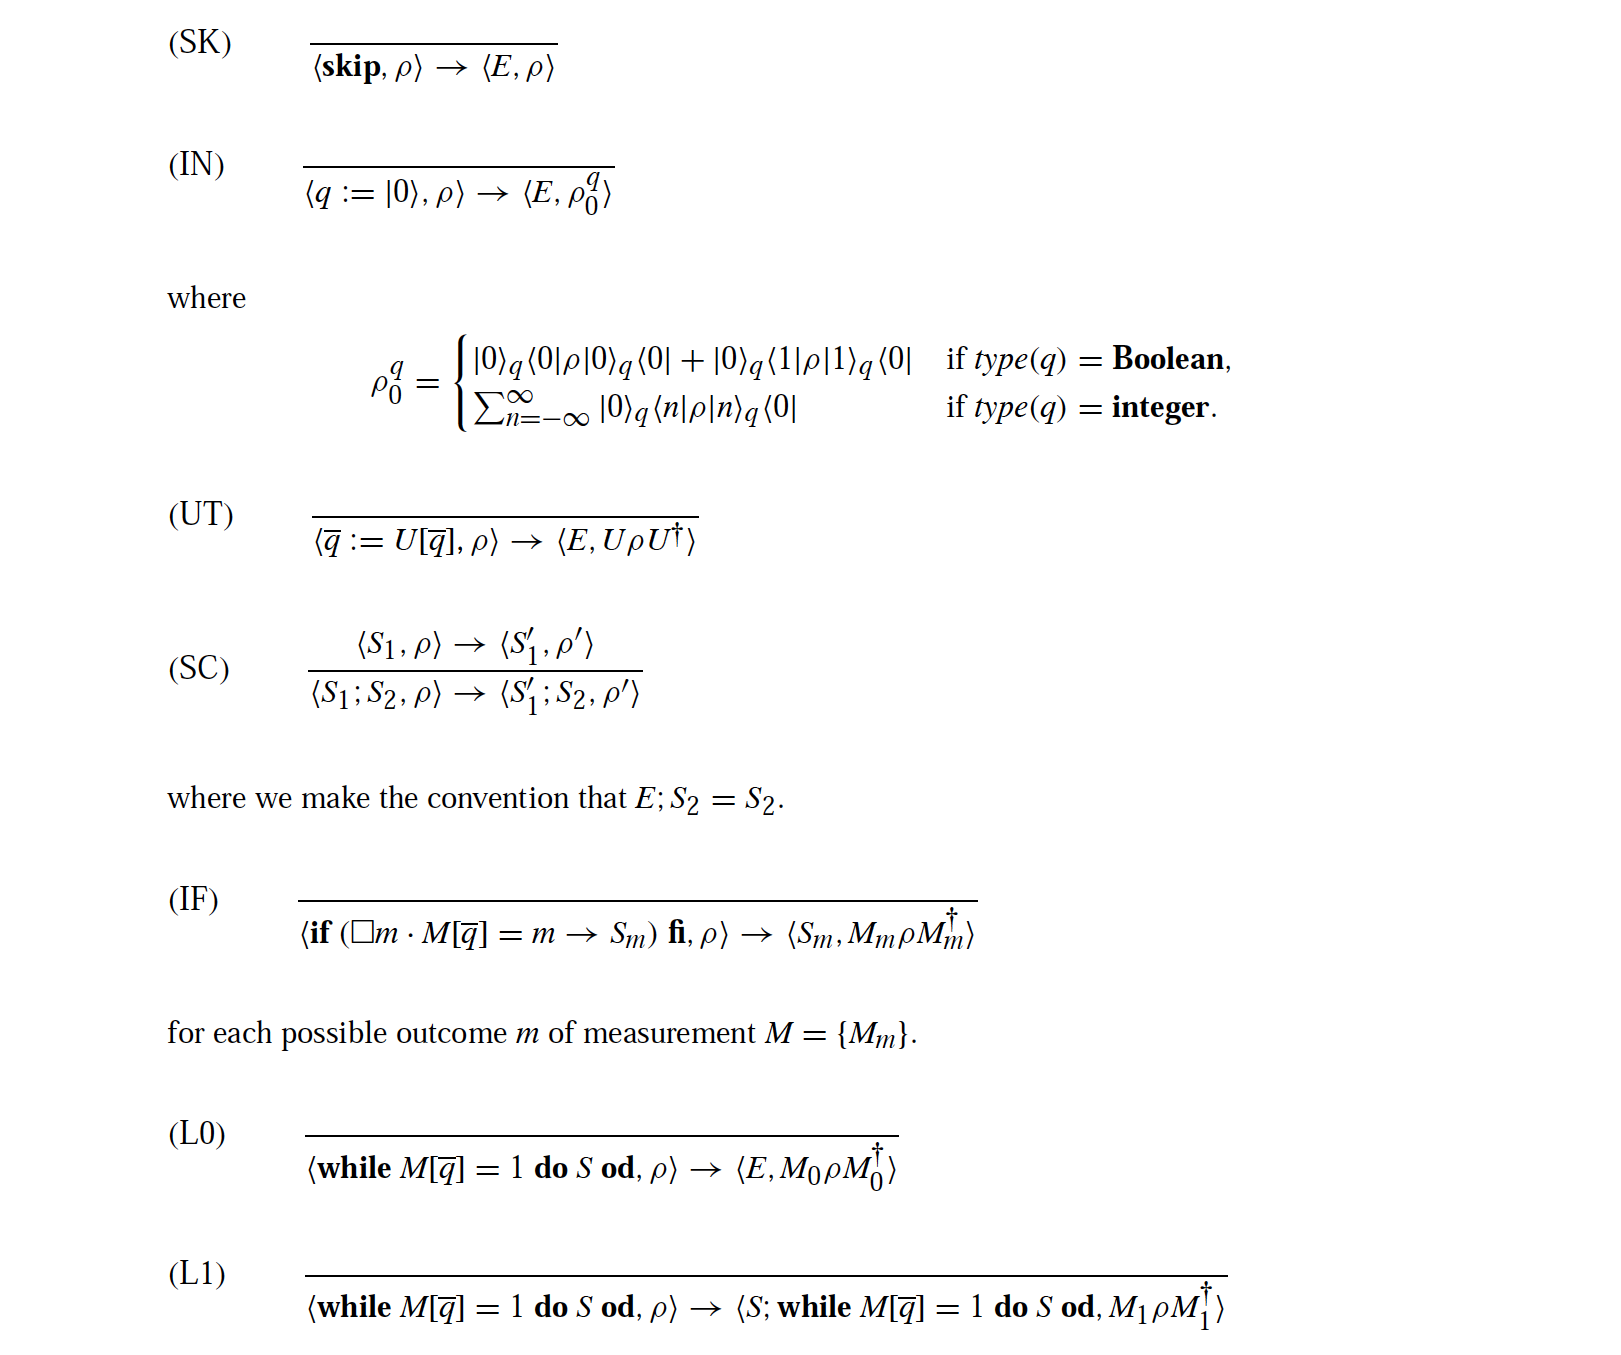
\includegraphics[height=0.75%93024
\textheight,width=%0.989184
0.71\textwidth]{Operational}%\caption{Transition Rules of Quantum \textbf{while}-Programs}
\end{figure}
}

\frame[t]{
\frametitle{Operational Semantics}
Remark:
\begin{enumerate}
    \item $E$ denotes the empty program, and $U\rho U^\dagger$ evolves the state $\rho$ with the unitary $U$;
    \pause 
    \item $\ket{0}_q$ $_q\bra{i}$ is tensored with identity on other qubits.
    \pause 
    \item When applying the IF rule, the program executes $S_{m_i}$ iff the measurement outcome is $m_i$, which occurs with probability $p_{m_i} = \tr(M_{m_i}\rho M_{m_i}^\dagger)$. 
    \pause 
    
    In this case, the post-measurement state (before executing $S_{m_i}$) is $\rho_{m_i} = \dfrac{M_{m_i}\rho M_{m_i}^\dagger}{p_{m_i}}$. Thus our IF rule is equivalent to: \begin{align*}
        \infer[(IF)]{(\qif{\square m\cdot M[\overline{q}]=m}{S_m})\xrightarrow{p_m} (S_m,\rho_m)}{}
    \end{align*}
    \pause 
    \item $L_0$ and $L_1$ describes the transition rules for exiting or continuing the loop respectively.
\end{enumerate}
}

\frame[t]{
\frametitle{Denotational Semantics}
Denote: 
\begin{enumerate}
    \item $\mathcal{H}_{all}:=$ the Hilbert space of all quantum variables, including those appearing in $\overline{q}$ and $S_m$.
    \item $\mathcal{D}(\mathcal{H}) := \{\rho\in \mathcal{H}\mid \tr(\rho)\leq 1\}$ ,the set of partial density operators in $\mathcal{H}$.
    \item $\to^* := $ the transitive and reflexive closure of $\to$. i.e., $\langle S,\rho\rangle\to^* \langle S',\rho'\rangle \iff$ $$ (\exists n\geq 0, \langle S_i, \rho_i\rangle) \langle S,\rho\rangle\to\langle S_1, \rho_1\rangle\to\cdots\to \langle S_{n-1}, \rho_{n-1}\rangle\to  \langle S',\rho'\rangle.$$
\end{enumerate}
\pause 

Like in classical cases, we define a semantic function $\sem{S}$ to reflex all states achievable from executing $S$ on state $\rho$ via different computational paths:
}




\frame[t]{
\frametitle{Denotational Semantics}
\begin{align*}
    \sem{S}:\dhall \to & \dhall,\\
    \rho\mapsto & \sum\{|\rho': \langle S,\rho\rangle\to^* \langle E,\rho'\rangle|\}
\end{align*}

where $\{|\cdot|\}$ denotes ``multiset'', i.e. a ``set'' with repetition.

We use multiset because the same partial density operator $\rho'$ may be obtained through different computational
paths.
\pause 
\begin{block}
{Linearity}Using induction on the structure of $S$, one may find that $\sem{S}$ is linear, i.e., for $\lambda_i\geq 0, \rho_i\in\dhall$, if $\sum_{i=1}^n\lambda_i\rho_i\in \dhall$, then:
$$\sem{S}(\sum_{i=1}^n\lambda_i\rho_i) = \sum_{i=1}^n\lambda_i\sem{S}(\rho_i)$$
\end{block}
}

\frame[t]{
\frametitle{Denotational Semantics}
E.g., for the following program: %where we apply Hadamard gate on quantum boolean variable $q:=\ket{0}$ and then perform a measurement in computational basis, 
\begin{figure}[H]\label{crg3}
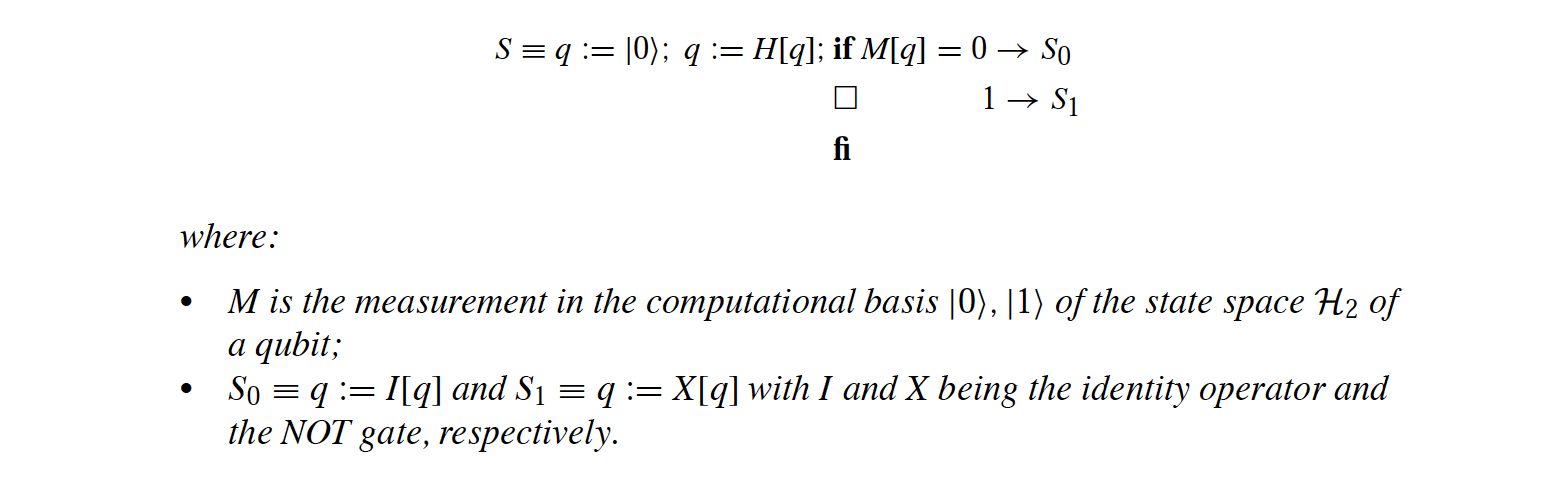
\includegraphics[height=0.45%93024
\textheight,width=%0.989184
1.05\textwidth]{OperationalEg}%\caption{Transition Rules of Quantum \textbf{while}-Programs}
\end{figure}

Denoting $\rho:=\ket{0}_{all}\bra{0}$, it can be computed that $\sem{S}(\rho) = \frac{1}{2}\rho + \frac{1}{2}\rho = \rho$. 
}

\frame[t]{
\frametitle{Denotational Semantics}
%\begin{block}{Complete Partial Order (CPO) on Operators and Quantum Operations}
\begin{itemize}
    \item Recall from our class that a CPO on a set $S$ is a partial order with a least element, s.t. for each increasing sequence $\{x_n\}$ there exists a least upper bound: $\bigsqcup_{n=0}^\infty x_n\in S$.\pause 
    \item For a Hilbert space $\H$, the \emph{L\"{o}wner order} $\sqsubseteq$ is defined on the set of linear operators on $\H$ (which by definition contains $\dhnall$) by $A\sqsubseteq B\iff B-A\succeq 0$ (i.e., $B-A$ is a positive semidefinite operator). \pause
    \item We denote by $\qoh$ the set of quantum operations in $\H$.\pause
\end{itemize}
With some effort one obtains: \footnote{For proof details, see Section $3.6$ of M. Ying, Foundations of Quantum Programming.}

%\end{block}
\begin{theorem}[CPO on $\dhnall$ and $\qoh$]
\begin{enumerate}
    \item $(\dhnall,\sqsubseteq)$ is a CPO with the least element $0_{\H}$.
    \item $\forall \E\in \qoh$, $\E$ is continuous on $\dhnall$.
    \item $(\qoh, \sqsubseteq_{q})$ is a CPO, with $\E\sqsubseteq_q\FF \iff \E(\rho)\sqsubseteq \FF(\rho) $ for all $\rho\in\dhnall$.
\end{enumerate}
\end{theorem}
}

\frame[t]{
\frametitle{Denotational Semantics: Structural Representation of Semantic Function}

Since a quantum program can be viewed as a sequence of quantum operations on $\dhall$, one may obtain the \textbf{while}-free structural representation of semantic functions using linearity (e.g., $\sem{\qif{\square m\cdot M[\overline{q}]=m}{S_m}}(\rho) =\sum_m \sem{S_m}(M_m\rho M^\dagger_m) ) $. 
\pause 

As for the \textbf{while}-loop, one performs an induction on the number of iterations and obtain:
$$
    \sem{while}  = \bigsqcup_{k=0}^\infty\sem{while^{k}}
$$
with $\sem{while^{k}}$ the $k$-th approximation of the loop: $$\sem{while^{k}}(\rho) = \sum_{n=0}^{k-1}\E_0\circ (\sem{S}\circ \E_1)(\rho) $$
where $$\E_i (\rho):= M_i\rho M^\dagger_i.$$
}

\frame[t]{
\frametitle{Denotational Semantics: Trace Non-increasing Property}
We conclude this section by the following finding, which may be proved using induction on the structure of quantum program $S$:\footnote{For details see Section $3.4$ of M. Ying, Foundations of Quantum Programming.}
\begin{theorem}
For any quantum program $S$ and any $\rho\in\dhall$, $\tr(\sem{S}(\rho))\leq \tr(\rho)$.
\end{theorem}

\pause

We also point out that the only way for a quantum program to diverge is to include a \textbf{while}-loop, in which case the divergence probability equals $$\tr(\rho)-\tr(\sem{S}(\rho)).$$
}
\end{document}























